\documentclass[border=3mm]{standalone}

\usepackage{tikz}
\usetikzlibrary{arrows.meta}

\begin{document}
	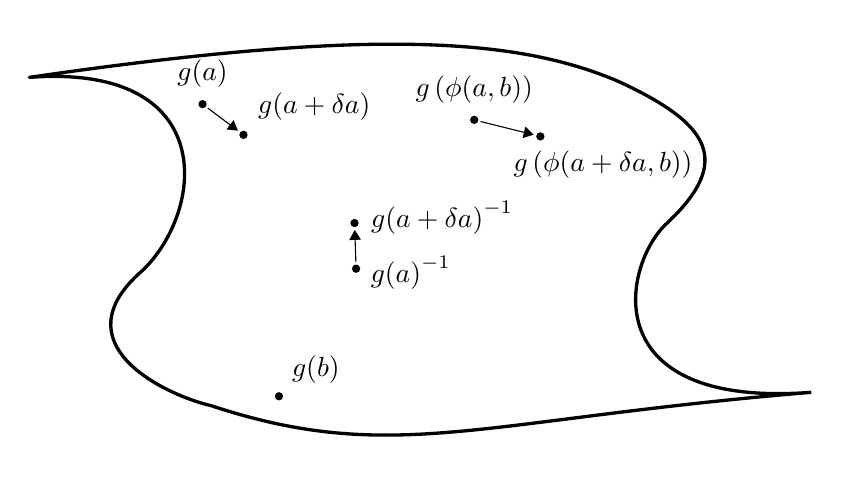
\begin{tikzpicture}[line cap=round]
		\draw[very thick] (-5.1,2.05) .. controls (-2.68,2.23) and (-2.87,0.36) .. (-3.66,-0.4) .. controls (-4.74,-1.33) and (-3.39,-1.98) .. (-2.79,-2.12) .. controls (-0.48,-2.88) and (0.6,-2.3) .. (4.83,-1.95) .. controls (2.05,-2.16) and (2.44,-0.31) .. (3,0.2) .. controls (3.84,0.99) and (3.54,1.46) .. (2.4,1.99) .. controls (1.05,2.58) and (-0.9,2.66) .. (-5.1,2.05);
		\node[fill,circle,inner sep=0pt,minimum size=3pt,label={above:$g(a)$},outer sep=1pt] (1) at (-2.9,1.71) {};
		\node[fill,circle,inner sep=0pt,minimum size=3pt,label={above right:$g(a+\delta a)$},outer sep=1pt] (2) at (-2.38,1.32) {};
		\node[fill,circle,inner sep=0pt,minimum size=3pt,label={above:$g\left(\phi(a,b)\right)$},outer sep=1pt] (3) at (0.55,1.51) {};
		\node[fill,circle,inner sep=0pt,minimum size=3pt,label={below right,xshift=-15pt:$g\left(\phi(a+\delta a,b)\right)$},outer sep=1pt] (4) at (1.39,1.3) {};
		\node[fill,circle,inner sep=0pt,minimum size=3pt,label={below right,yshift=10pt:${g(a)}^{-1}$},outer sep=1pt] (5) at (-0.95,-0.38) {};
		\node[fill,circle,inner sep=0pt,minimum size=3pt,label={right,yshift=2pt:${g(a+\delta a)}^{-1}$},outer sep=1pt] (6) at (-0.97,0.2) {};
		\node[fill,circle,inner sep=0pt,minimum size=3pt,label={above right:$g(b)$}] at (-1.93,-2) {};
		\draw[-Triangle] (1) -- (2);
		\draw[-Triangle] (3) -- (4);
		\draw[-Triangle] (5) -- (6);
	\end{tikzpicture}
\end{document}